\documentclass[tikz,border=2pt]{standalone}
\usepackage{amsmath}
\usetikzlibrary{arrows.meta}
\begin{document}
% wmean <- function(x, w = NULL) with x = c(2, 4, 9): without w the default NULL is used and
% is.null(w) is TRUE, giving the mean 5; with w = c(0.5, 0.25, 0.25) the weighted mean 4.25.
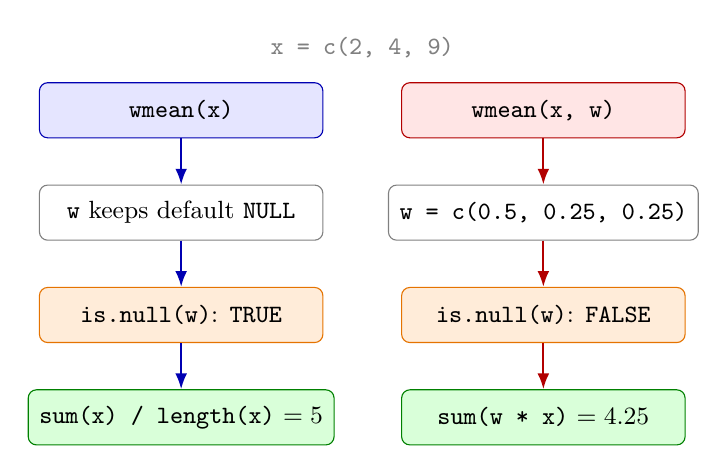
\begin{tikzpicture}[font=\small, >={Latex[length=2mm]},
  box/.style={draw, rounded corners=3pt, align=center, inner sep=4pt, minimum width=3.6cm, minimum height=7mm}]
  \node[box, draw=blue!70!black, fill=blue!10, font=\small\ttfamily] (c1) at (0,0) {wmean(x)};
  \node[box, draw=red!70!black, fill=red!10, font=\small\ttfamily] (c2) at (4.6,0) {wmean(x, w)};
  \node[box, draw=gray] (w1) at (0,-1.3) {\texttt{w} keeps default \texttt{NULL}};
  \node[box, draw=gray] (w2) at (4.6,-1.3) {\texttt{w = c(0.5, 0.25, 0.25)}};
  \node[box, draw=orange!90!black, fill=orange!15] (t1) at (0,-2.6) {\texttt{is.null(w)}: \texttt{TRUE}};
  \node[box, draw=orange!90!black, fill=orange!15] (t2) at (4.6,-2.6) {\texttt{is.null(w)}: \texttt{FALSE}};
  \node[box, draw=green!50!black, fill=green!15] (r1) at (0,-3.9) {\texttt{sum(x) / length(x)} $=5$};
  \node[box, draw=green!50!black, fill=green!15] (r2) at (4.6,-3.9) {\texttt{sum(w * x)} $=4.25$};
  \foreach \a/\b in {c1/w1,w1/t1,t1/r1} \draw[->, thick, blue!70!black] (\a) -- (\b);
  \foreach \a/\b in {c2/w2,w2/t2,t2/r2} \draw[->, thick, red!70!black] (\a) -- (\b);
  \node[gray] at (2.3,0.8) {\texttt{x = c(2, 4, 9)}};
\end{tikzpicture}
\end{document}
